\hyt{acrosstheuniverse}
\song{Across the Universe} \interpret{beatles}{The Beatles}

\note{\footnote{Na albu Let It Be byla tato píseň dodatečně zpomalena a tím transponována do tóniny C\kk dur.}}

\intro{

\vspace{-45pt}
\hspace{20pt}	
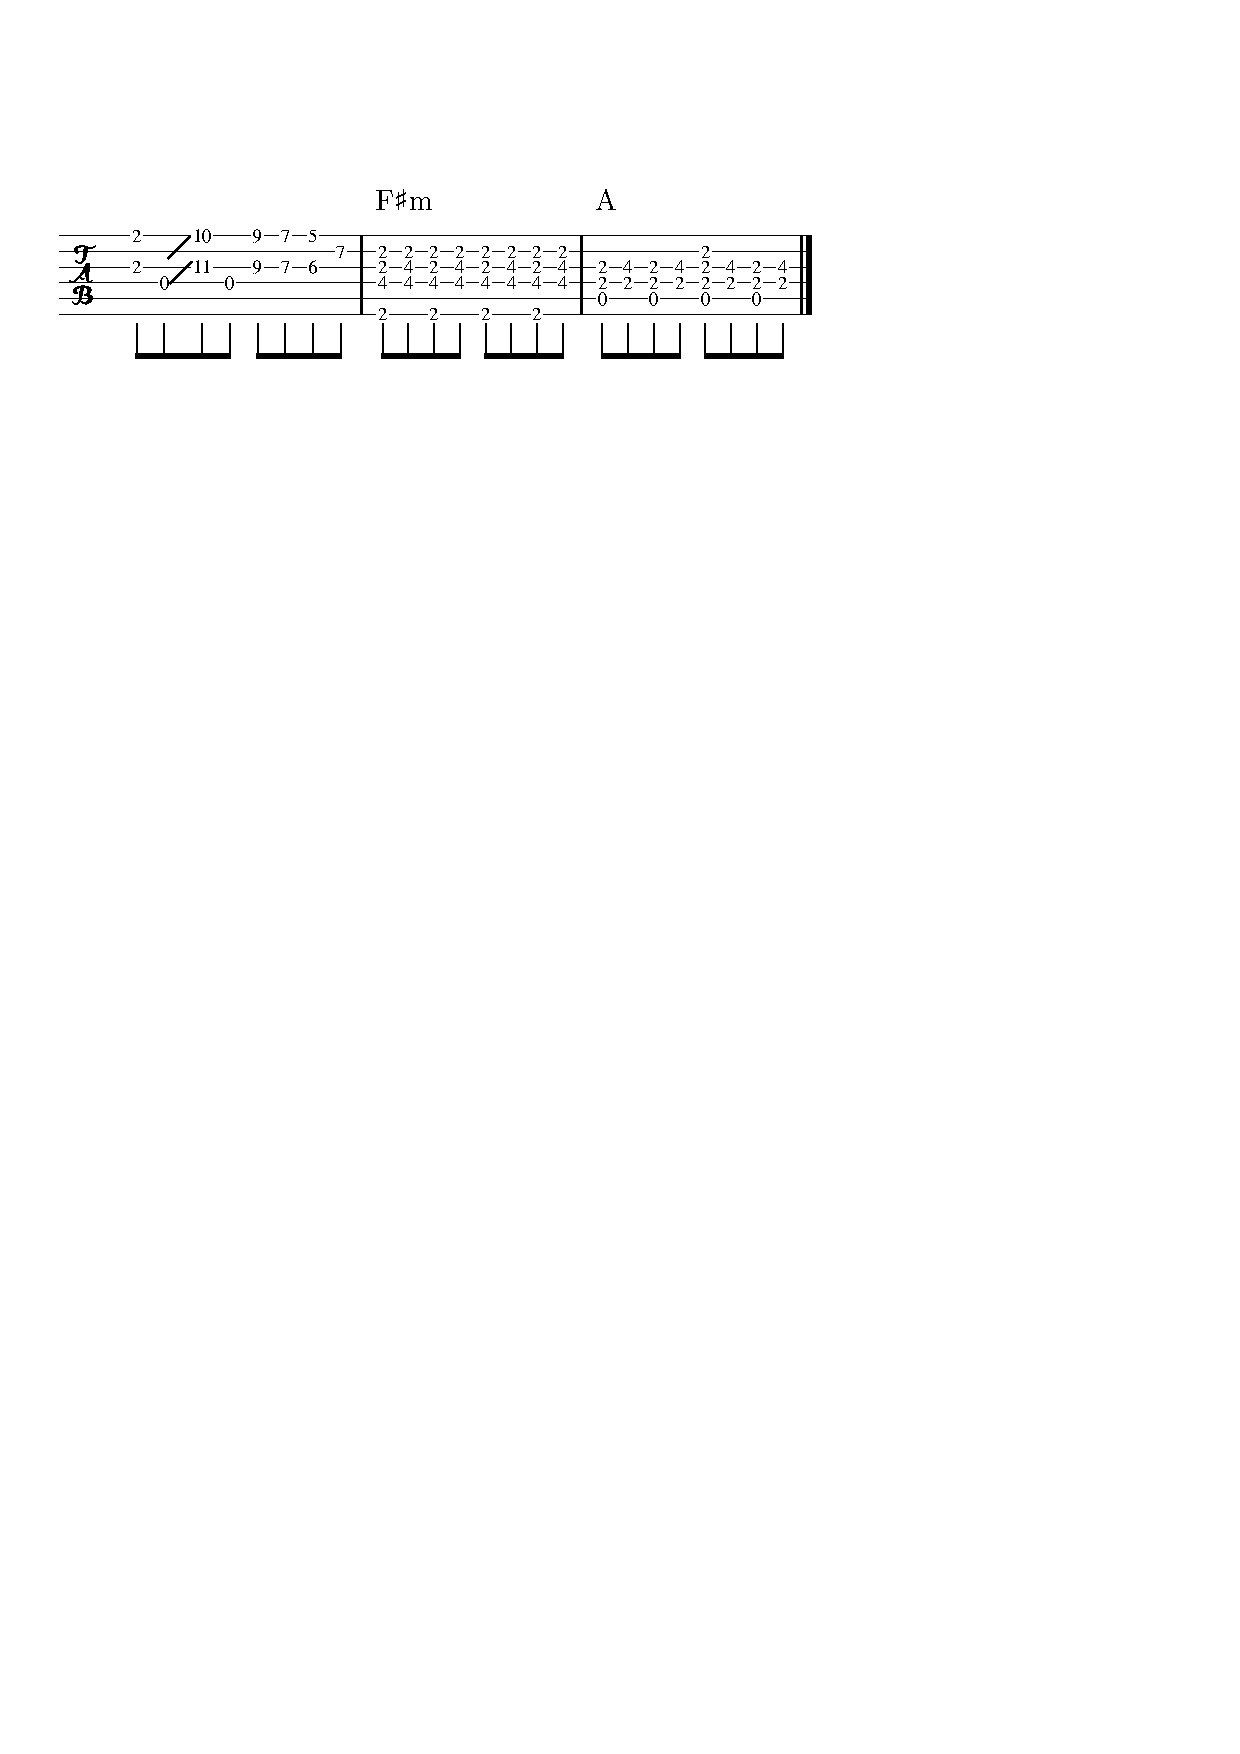
\includegraphics[width=515pt]{scores/acrosstheuniverse.pdf}
}
\ns
\vspace{-10pt}

\vers{1}{
\chord{D}Words are flowing \chord{Hm}out like endless \chord{F\kk m}rain into a paper cup, they\\
\chord{Em}slither while they pass the slip a\chord{A}way across the Universe.\\
\chord{D}Pools of sorrow, \chord{Hm}waves of joy are \chord{F\kk m}drifting through my open mind,\\
po\chord{Em}ssessing and ca\chord{Gm}ressing me.
}
\ns

\refrain{
\chord{D}Jai Guru Deva, \chord{A}om\footnote{Hinduistická mantra. Přibližný překlad: \textit{Jai} -- \uv{Budiž sláva}, \textit{Guru} -- \uv{učitel}, \textit{Deva} -- \uv{boží}, dohromady tedy volně přeloženo, \uv{Budiž sláva duchovnímu mistru.} Toto byla Johnova mantra, která mu pomáhala se soustředit během meditace. Pravděpodobně byla inspirována Maharišim, indickým filosofem, se kterým Beatles strávili v roce 1968 několik týdnů a jehož učitelem byl Brahmananda Saraswati, známý též jako Guru Déva.}\dots\\
\rep{\chord{A}Nothing's gonna change my \chord{A\7}world, \chord{G}nothing's gonna change my \chord{D}world.}
}
\ns

\vers{2}{
\chord{D}Images of \chord{Hm}broken light, which \chord{F\kk m}dance before me like a million\\
\chord{Em}eyes, they call me on and on a\chord{A}cross the Universe.\\
\chord{D}Thoughts meander \chord{Hm}like a restless \chord{F\kk m}wind inside a letterbox, they\\
\chord{Em}tumble blindly as they make their \chord{A}way across the Universe.
} \refsm{}
\ns

\vers{3}{
\chord{D}Sounds of laughter, \chord{Hm}shades of earth are \chord{F\kk m}ringing through my open views,\\
in\chord{Em}citing and in\chord{Gm}viting me.\\
\chord{D}Limitless, un\chord{Hm}dying love, which \chord{F\kk m}shines around me like a million\\
\chord{Em}suns and calls me on and on a\chord{A}cross the Universe.
} \refsm{}

\cod{
\rep{\chord{D}Jai Guru Deva.} \note{fade out}
}
\newpage
